%======================================================================
\section{Conditioning generation on PCA coordinates}\label{sec:cond}
%======================================================================
An earlier version of this project steered generation by appending the discretised PCA coordinates
to every sequence as two extra Potts sites and amplifying their couplings by a factor
$\beta_\mathrm{PCA}$ at sampling time; steering only began around $\beta_\mathrm{PCA}\approx10$, and
beyond it the samples drifted past the target and lost the HPD motif. Here we test two
alternatives, both built on one exact property of the PCA used throughout this report. The full
study, including a slower derivation, is in the companion note \texttt{conditional.pdf}.

\paragraph{A PCA coordinate is an exact Potts term.} The PCA is fitted on one-hot vectors, so once
fitted a coordinate is a projection, and because a one-hot sequence has a single $1$ per site the
projection reduces to one table entry per site:
\begin{equation}
\mathrm{PC}_c(\bm x)=\sum_{i}V_c(i,x_i)-m_c .
\end{equation}
Squaring a sum of per-site terms produces per-site and pairwise terms, so the harmonic restraint
\begin{equation}
E_\lambda(\bm x)=E(\bm x)+\frac{\lambda}{2}\sum_c\big(\mathrm{PC}_c(\bm x)-t_c\big)^2
\label{eq:restraint}
\end{equation}
is itself a Potts energy, with coupling correction $\Delta J_{ij}(a,b)=-\lambda\sum_cV_c(i,a)V_c(j,b)$
and a field linear in the target $\bm t$. Its Boltzmann distribution is $p(\bm x)$ times a Gaussian
window of width $1/\sqrt\lambda$ around $\bm t$, i.e.\ exactly the posterior of $\bm x$ given a noisy
measurement $\mathrm{PC}(\bm x)\approx\bm t$.

\paragraph{Two methods.} \textbf{C1} adds \eqref{eq:restraint} to the trained model at sampling time:
each site update also scores how far each candidate letter would put the coordinate from $\bm t$.
Nothing is retrained. \textbf{C3} learns the conditional instead: fields
$h_i(a\mid\bm z)=\sum_fW_f(i,a)\phi_f(\bm z)$ with $\phi=(1,u_1,u_2,u_1^2,u_2^2,u_1u_2)$ ($\bm u$ the
standardised coordinates) are trained jointly with the couplings by conditional pseudo-likelihood on
pairs $(\bm x,\mathrm{PC}(\bm x)+\sigma\bm\epsilon)$, then sampled at $\bm z=\bm t$. Trained on
coordinates blurred by $\sigma$, C3 is fitted to the same distribution C1 writes down with
$\lambda=1/\sigma^2$; we use $\sigma=1,0.5,0.25$ to match $\lambda=1,4,16$. Optionally a gain $\kappa$
multiplies the $\bm z$-dependent field at sampling time --- the analogue of $\beta_\mathrm{PCA}$.

\paragraph{Setup.} Targets are the three cluster centres of \S\ref{sec:gen} (\MissCl, the
under-sampled HscB-like group, and the two others). For each method, target and setting, $3000$
chains start from random training sequences and run $500$ sweeps; the restrained chains converge in
$50$--$100$ sweeps. Quality is measured against the natural test sequences of the target cluster,
with every pool (including the natural ceiling) evaluated at the same size of $3000$ because $C_{ij}$
estimates are noisy. Both methods use the same field-free model, trained with longer patience
(best epoch \EpBase\ instead of \EpClean).

\paragraph{A caveat on mode weights uncovered on the way.} That longer-trained model has a slightly
better validation pseudo-likelihood (\ValBase\ vs \ValClean\ nats per sequence) but samples the
three clusters in proportions \ShareBasep\ (C0/C1/C2, \%) instead of \ShareClean\ for the model of
the previous sections (natural \ShareNat). Retraining the earlier model reproduces its couplings bit
for bit, so the only difference is $294$ epochs of training: the C1/C2 balance moved by $2.7$ nats of
free energy for $0.2$ nats of pseudo-likelihood. The good coverage of the two major clusters reported
above is therefore a property of that checkpoint, not a robust property of pseudo-likelihood
training; the deficit of \MissCl\ is present in every model trained.

\begin{figure}[t]\centering
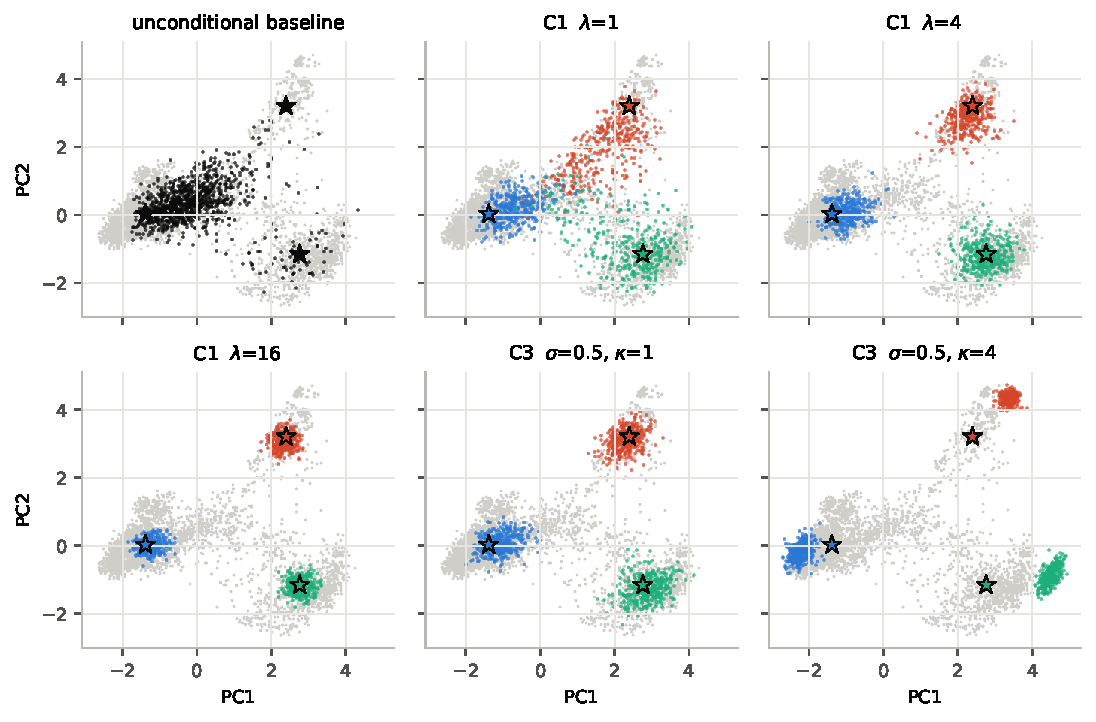
\includegraphics[width=0.84\linewidth]{../outputs/figures/cond_pca.pdf}
\caption{Conditioned samples in the PCA plane (grey: natural test). Stars: targets; points are
coloured by the target they were aimed at. Top left: unconditional sampling, which visits C1 almost
exclusively. Bottom right: C3 with its target field amplified ($\kappa=4$) --- every pool lands
beyond its target.}
\label{fig:condpca}
\end{figure}

\begin{table}[t]\centering\small\setlength{\tabcolsep}{4pt}
\begin{tabular}{lccccc}
\toprule
 & in target (\%) & distance & $r(C_{ij})$ & HPD (\%) & diversity \\
\midrule
unconditional baseline & 5/86/10 & 3.9/1.5/3.3 & 0.16/0.42/0.34 & 99/99/99 & 0.62/0.62/0.62 \\
rejection from baseline & 100/100/100 & 1.8/1.2/1.2 & 0.25/0.50/0.49 & 97/99/98 & 0.69/0.59/0.68 \\
\midrule
C1 $\lambda{=}1$ & 80/100/88 & 1.6/0.9/1.0 & 0.44/0.47/0.57 & 96/99/98 & 0.70/0.56/0.65 \\
C1 $\lambda{=}4$ & 100/100/100 & 0.6/0.5/0.5 & 0.46/0.39/0.60 & 96/99/99 & 0.64/0.52/0.62 \\
C1 $\lambda{=}16$ & 100/100/100 & 0.3/0.3/0.3 & 0.37/0.30/0.54 & 96/99/98 & 0.61/0.48/0.61 \\
\midrule
C3 $\sigma{=}1$ & 100/100/100 & 0.7/0.9/0.7 & 0.47/0.48/0.64 & 100/99/99 & 0.63/0.56/0.62 \\
C3 $\sigma{=}0.5$ & 100/100/100 & 0.4/0.5/0.5 & 0.38/0.40/0.60 & 100/100/100 & 0.57/0.52/0.61 \\
C3 $\sigma{=}0.25$ & 100/100/100 & 0.3/0.3/0.4 & 0.33/0.34/0.56 & 100/99/99 & 0.56/0.48/0.60 \\
\midrule
C3 $\sigma{=}0.5$, $\kappa{=}4$ & 100/100/100 & 1.5/0.9/1.8 & 0.12/0.18/0.29 & 100/100/92 & 0.29/0.31/0.55 \\
C3 $\sigma{=}0.5$, $\kappa{=}8$ & 100/100/100 & 1.6/1.2/1.8 & 0.08/0.08/0.12 & 100/100/56 & 0.16/0.21/0.40 \\
\midrule
natural (ceiling) & 100/100/100 & 1.0/1.3/0.8 & 0.66/0.63/0.75 & 100/100/99 & 0.67/0.60/0.64 \\
\bottomrule
\end{tabular}

\caption{Conditioning on each of the three cluster centres; each entry lists C0/C1/C2. In target:
fraction of samples landing in the target cluster. Distance: mean $\|\mathrm{PC}-\bm t\|$.
$r(C_{ij})$: against the natural test sequences of the target cluster. HPD: fraction retaining the
J-domain HPD motif. Diversity: mean pairwise Hamming distance within the pool. Rejection keeps the
unconditional samples that fall in the cluster ($496$, $3000$, $948$ sequences). Ceiling: $3000$
natural training sequences of the cluster.}
\label{tab:cond}
\end{table}

\paragraph{C1 steers to every target, including the neglected one, and keeps the protein.} Without
the restraint, $5\%$ of the chains reach \MissCl; from $\lambda=4$ on, all of them do
(Table~\ref{tab:cond}, Figure~\ref{fig:condpca}). The distance to the target falls as
$1/\sqrt\lambda$, the width of the Gaussian window, and responds monotonically to $\lambda$. The HPD
motif is retained in $96$--$99\%$ of samples at every $\lambda$. The covariation agreement peaks at
$\lambda\approx1$--$4$ (e.g.\ $r(C_{ij})=\ConeALfourrC$ for C0 and $0.60$ for C2 at $\lambda=4$,
ceilings \CeilA\ and \CeilC) and decreases for stiffer restraints, mainly because a window much
narrower than a natural cluster (radius ${\sim}1$) samples the cluster's centre and loses its
internal variation. Rejection sampling, the exact conditional, needs $10\,000$ unconditional samples
to produce $496$ in C0; C1 at $\lambda=4$ produces C0 sequences of the same energy (\ConeALfourE\ vs
$-106.0$), as expected if it samples the model's own conditional. That energy is $14$ units above the
natural C0 sequences (\NatEA): C1 reaches the neglected region but inherits the model's view of it.

\paragraph{C3 matches C1 at $\lambda=1/\sigma^2$, and does better on the neglected cluster.} At
$\kappa=1$ C3 lands on target with the accuracy and quality of C1 at the matching stiffness
(Table~\ref{tab:cond}), as the equivalence above predicts. The one systematic difference is
\MissCl: C3 gets there at weak conditioning where C1 stops short (distance $0.74$ vs $1.59$ at
$\sigma=1$/$\lambda=1$), and its C0 sequences have lower energy (\CthreeAsHKoneE\ vs \ConeALfourE),
closer to the natural ones. C1 reweights the unconditional model, which carries the free-energy
error of Table~\ref{tab:clusene}; C3 learned the conditional from data and does not inherit it.

\paragraph{Amplifying the target field reproduces the earlier failure.} With $\kappa=2,4,8$ the samples
overshoot the target by up to $1.5$ PC units, diversity collapses towards copies of a single
sequence ($0.16$ for C0 at $\kappa=8$), $r(C_{ij})$ drops to $0.1$, and for C2 the HPD motif is lost in
$44\%$ of the samples. The cause follows from the expansion of \eqref{eq:restraint}: the exact
conditional pairs a field that pushes towards $\bm t$ with a coupling term that holds the coordinate
\emph{at} $\bm t$; $\kappa$ (like $\beta_\mathrm{PCA}$) amplifies the push without the spring. This is
the ``drifts past the target, loses the HPD motif'' behaviour of the earlier study, now explained.

\begin{figure}[t]\centering
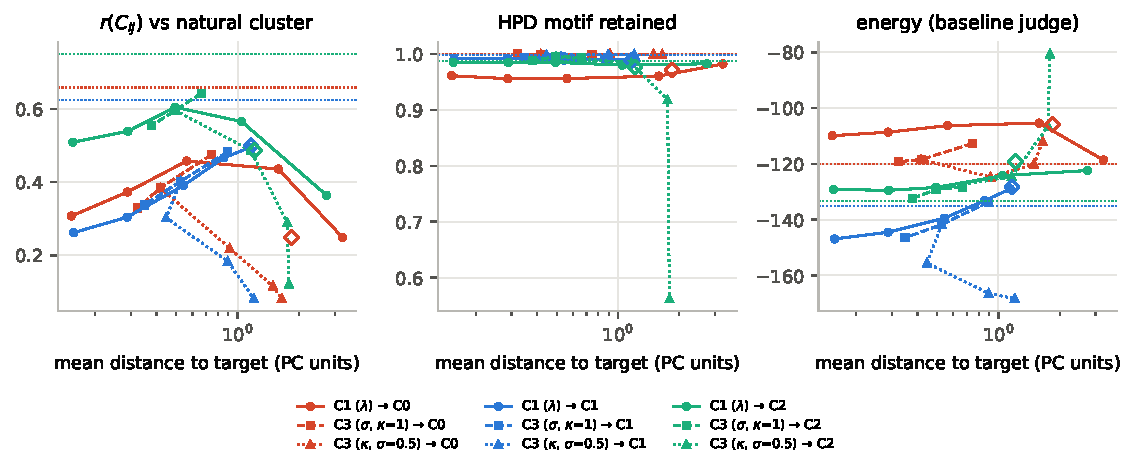
\includegraphics[width=\linewidth]{../outputs/figures/cond_tradeoff.pdf}
\caption{Accuracy--quality trade-off per method (line style) and target (colour). Solid circles: C1,
$\lambda=0.25\to64$ (right to left). Dashed squares: C3 at $\kappa=1$, $\sigma=1\to0.25$. Dotted
triangles: C3 at $\sigma=0.5$, $\kappa=1\to8$. Open diamonds: rejection. Dotted horizontal lines:
natural ceiling ($r(C_{ij})$) or natural cluster value (HPD, energy under the baseline model).}
\label{fig:condtrade}
\end{figure}
